\documentclass[11pt]{article}  % include bezier curves
\renewcommand\baselinestretch{1.0}           % single space

\oddsidemargin -10 true pt      % Left margin on odd-numbered pages.
\evensidemargin 10 true pt      % Left margin on even-numbered pages.
\marginparwidth 1.5 true in    % Width of marginal notes.
\oddsidemargin  0 true in       % Note that \oddsidemargin=\evensidemargin
\evensidemargin 0 true in
\topmargin -0.5 true in        % Nominal distance from top of page to top of
\textheight 9.0 true in         % Height of text (including footnotes and figures)
\textwidth 6.5 true in        % Width of text line.
\parindent=0pt                  % Do not indent paragraphs
\parskip=0.15 true in
%\usepackage{color}              % Need the color package
\usepackage{hyperref}
\usepackage[pdftex]{color, graphicx}
%\usepackage{graphicx} %for epsfig
\usepackage{graphics}
\usepackage{subfig}
\usepackage{epsfig}
\usepackage{latexsym}
\usepackage{mathrsfs}
\usepackage{eufrak}
\usepackage{amsmath}
\usepackage{graphicx}
\usepackage{longtable}
\usepackage{afterpage}


\title{M3D-C1: Current Status and Future Development in Mode Switch}
\author{Fan Zhang, Seegyoung Seol, Mark S. Shephard} 
\begin{document} 
\maketitle

\tableofcontents
\clearpage
\section{Introduction}
This document overviews the current status of the software that SCOREC provides to M3D-C1 \cite{jardin2004triangular,jardin2007high,ferraro2009calculations,jardin2012review,jardin2012multiple, Ferraro2011, Ferraro2014} and the requirements of the new capability that enables M3D-C1 to switch between  modes. M3D-C1  applies C$^1$  4$^{th}$ order element to solve the magnetohydrodynamics (MHD) equations and simulates the nonlinear instability of the plasma in the tokamak.  The case of non-axis-symmetric instability requires the simulation to be performed on the 3D mesh.  The new  capability  to be developed will allow  M3D-C1  to start with a 2D analysis and switch to 3D when a full 3D discretization is needed.  

The software structure of M3D-C1 is illustrated by Fig. \ref{fig:structure}. The  mesh infrastructure \cite{pumi-web-page,Seol2014} provides the interface to define the geometric model of the tokamak and manages the database of the distributed mesh. The original PDE is discretized over the mesh entities by the Galerkin finite element method \cite{jardin2004triangular,jardin2007high,ferraro2009calculations,jardin2012review,jardin2012multiple}. The element contribution to the stiffness matrix and the force vector \cite{hughes2012finite} is integrated over mesh elements. The mesh infrastructure provides the element connectivity and the geometric information during the discretization of PDE over elements. The global discrete equation is formed from the element-level discrete equation. The DOF ordering is calculated and the global system of the equations is assembled. The parallel communication during the assembly is performed through the localized inter-process communication based on the mesh partition \cite{sahni2009strong,ovcharenko2012neighborhood}.  The global discrete system is solved through the linkage to the equation solvers such as SuperLu \cite{superlu_ug99} and PETSc \cite{petsc-web-page}. There is the procedure that assess the solution quality and improve the mesh if needed through local mesh modification \cite{li20053d,sahni2007automated, lu2013parallel}.

\begin{figure}[hbt]
\center

\includegraphics[width=0.6\textwidth]{fig/m3dc1Structure.png}
\caption{Software structure of M3D-C1} \label{fig:structure}
\end{figure}

The SCOREC group provides the underlying mesh infrastructure, the mesh improvement capability, and the procedures to interact with the mesh infrastructure. The following sections discuses the current capabilities that The SCOREC group provides and the new capability to be developed to support the mode switch in M3D-C1. Section \ref{sec:geo} discusses the tokamak geometry definition in M3D-C1.  Section \ref{sec:mesh} discusses the meshing capabilities of M3D-C1. Section \ref{sec:parallel} discusses the procedures that interact with mesh infrastructure.  Section \ref{sec:futuredevelop} discuses the future development to support the mode switch of M3D-C1. An appendix is provided that describes the function list and verification tools.
\section{Geometry Definition}  \label{sec:geo}
This section describes the geometric components of the tokamak that need to be constructed in M3D-C1. 
The complete geometry is defined by the topological structure and the shape information of the geometric entities. 
\subsection{Geometric Description of the Tokamak}
Tokamak fusion reactors \cite{wesson2011tokamaks} are applied as the experimental approach to study magnetically confined sustainable fusion reactions. The basic tokamak is a torus that is symmetric along
the toroidal direction. The fusion material in a tokamak exists as the state of plasma which is confined by the magnetic field \cite{chen1984introduction}.  M3D-C1 studies the behaviors
of plasma in tokamaks.

Fig. \ref{fig:geo} illustrates the geometric components of the tokamak cross section \cite{wesson2011tokamaks,stacey1982fusion}.  Two coordinate systems,  $(R,Z,\varphi)$ and $(r,\theta, \varphi)$, are  applied in the torkamak geometry. $R$ is the major radius that measures the distance to the axis of the torus. $r$ is the minor radius that measures the distance to the magnetic axis on the cross section. $\varphi$ and $\theta$ are toroidal and poloidal angles respectively. 
The plasma region (9 in Fig. \ref{fig:geo}) is bounded by the limiter or the boundary of the material wall (12 in Fig. \ref{fig:geo}) \cite{wesson2011tokamaks}. There exists a separatrix or the last closed flux surface in plasma (3 in Fig. \ref{fig:geo}) and  it further splits the region into two distinct regions: the plasma core and the scraped-off layer (5 and 4 in Fig. \ref{fig:geo}) \cite{wesson2011tokamaks}. The flux surfaces in the plasma core are concentric loops between the magnetic axis (0 in Fig. \ref{fig:geo}) and the separatrix. The surfaces are distorted away by the x point (6 in Fig. \ref{fig:geo}) which is a saddle point of the magnetic flux on the separatrix.  There can be more than one x points existing on the separatrix in more general situations. The scrape-off layer is the region between the separatrix and the wall boundary. Flux surfaces end at the wall in this region and the outermost surface coincide with the wall.  In addition to the plasma region, the components of the geometry can also include the wall region and an vacuum vessel (8 and 7 in Fig. \ref{fig:geo}).  

\begin{figure}[htb]
\center
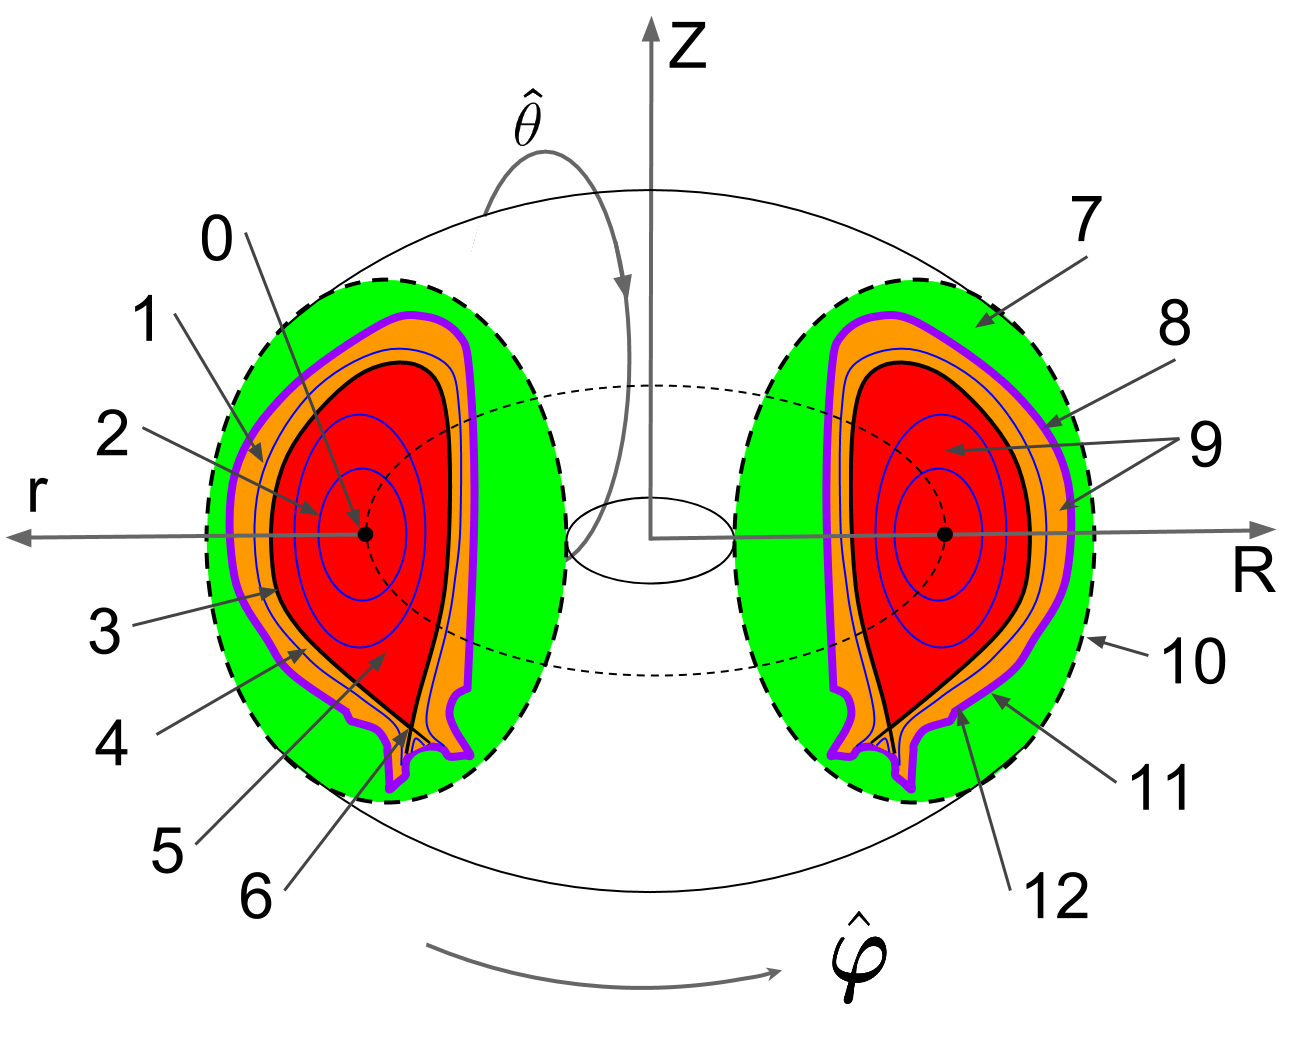
\includegraphics[width=\textwidth]{fig/fusiongeo3d.png}
\caption{Geometric components of the fusion reactor. The coordinate system is $(R,Z, \varphi)$ or $(r,\theta, \varphi)$, where $R$ and $r$ are major and minor radii, and $\varphi$ and $\theta$ are toroidal and poloidal angles. The components include magnetic axis (0), open flux surface (1), closed flux surface (2),  separatrix (3), scrape-off layer (4), plasma core (5), x point (6), vacuum vessel (7), wall region (8),  plasma region (9), vacuum boundary (10), outer wall boundary (11), and inner wall boundary (12).} \label{fig:geo}
\end{figure}

The geometry applied in M3D-C1 is the 3D torus made up by the plasma region, the material wall and the vacuum vessel.  There are planes placed around the torus axis and each plane forms a cross section of the tokamak.
\clearpage
\subsection{Geometry Model Definition in M3D-C1}
The geometric model is defined in terms of the abstraction of the topological entities and their adjacencies \cite{weiler1986topo}. The information that defines the shape of the model entities is associated with the topological entitles. 

The topological entities of the tokamak are regions, that are bounded by shells, which are made up by faces, that are bounded by loops, which are made up of edges, that are bounded by vertices. The topological structure of the geometry entities is summarized below.
\begin{itemize}
\item The 3D torus is made up by regions between the planes (Fig. \ref{fig:3dtopo}). There are up to three regions between two planes that correspond to the  plasma, the wall and vacuum in the tokamak reactor (9, 8 and 7 in Fig. \ref{fig:geo}). 
\begin{figure}[htb]
\center
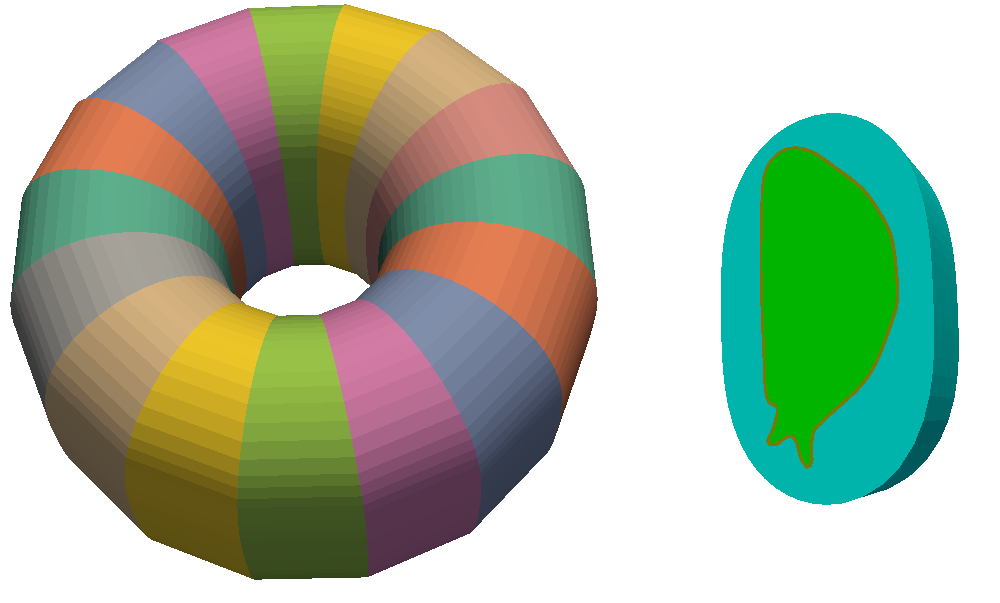
\includegraphics[width=0.8\textwidth]{fig/3dGeoTorus.png}
\caption{The 3D torus with 16 planes. The regions between planes correspond to the plasma, wall and vacuum in Fig. \ref{fig:geo}.} \label{fig:3dtopo}
\end{figure}

\item A region is bounded by a shell that is made up of two faces on the neighboring planes and a number of faces between planes (Fig. \ref{fig:regiontopo}). The faces between planes are on the boundaries of the material wall or the vacuum (12, 11 and 10 in Fig. \ref{fig:geo}). The geometry is non-manifold \cite{weiler1986topo} that each face except that on the vacuum boundary is used to form two regions. 
\begin{figure}[htb]
\center
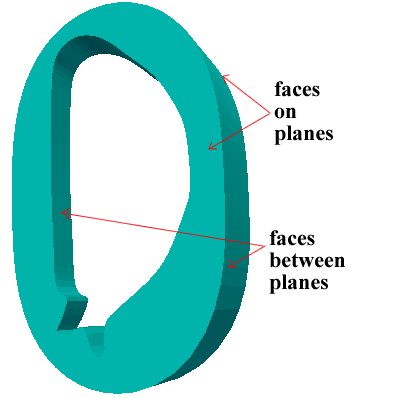
\includegraphics[width=0.4\textwidth]{fig/vacuumGeoRegionFace.png}
\caption{The geometric region of the vacuum between two planes} \label{fig:regiontopo}
\end{figure}

\item There are three faces on a plane (Fig. \ref{fig:facetopo}). The inner  plasma face is bounded by the loop on the inner material wall (loop 1 in Fig. \ref{fig:facetopo}). The wall face is bounded by two loops on the inner and outer material walls (loop 1' and loop 2 in Fig. \ref{fig:facetopo}). The outer vacuum face is bounded by the loop on the outer material wall and the loop on the vacuum vessel (loop 2' and loop 3 in Fig. \ref{fig:facetopo}). The loops that two faces contact on the plane are formed by the same group of edges in the opposite directions. 
\begin{figure}[htb]
\center
\begin{tabular}{ccc}
\subfloat[plasma face]{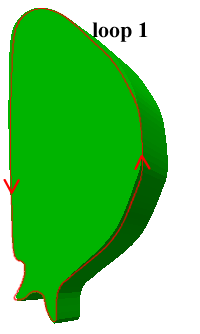
\includegraphics[scale=0.4]{fig/plasmaGeoRegion.png}}
 & \subfloat[wall face]{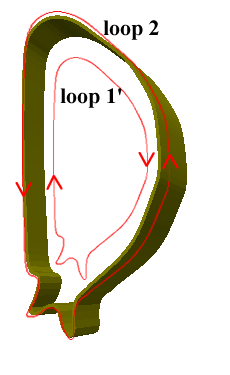
\includegraphics[scale=0.4]{fig/wallGeoRegion.png}}
 & \subfloat[vacuum face]{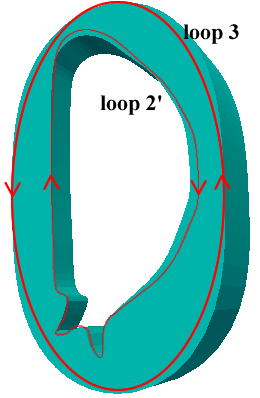
\includegraphics[scale=0.4]{fig/vacuumGeoRegion.png}}
\end{tabular}
\caption{Geometric faces on the plane} \label{fig:facetopo}
\end{figure}

\item The face between planes (Fig. \ref{fig:facetopobtw}) is either bounded by one loop that are made up of two edges on the planes and  two edges between planes, or two loops on the planes.
\end{itemize}
\begin{figure}[htb]
\center
\begin{tabular}{cc}
\subfloat[face bounded by one loop]{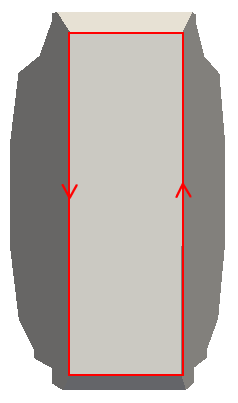
\includegraphics[scale=0.5]{fig/facebtw1.png}}
 & \subfloat[face bounded by two loops]{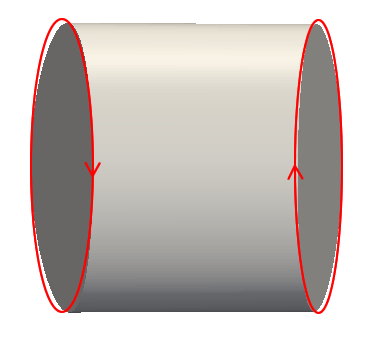
\includegraphics[scale=0.5]{fig/facebtw2.png}}
\end{tabular}
\caption{Geometric faces between planes} \label{fig:facetopobtw}
\end{figure}

In addition to the topological structure, the shape information defines the complete geometry model of the tokamak  geometry. The shape information are the positions of the model vertices, the geometry of the curves associated with the model edges, and the geometry of the surfaces associated with the model faces.  Ideally the geometry of the wall curves would be that defined in the reactor's CAD model. Currently the wall curves is defined by an ordered set of points and the points are interpolated by the B-splines \cite{prautzsch2002bezier}. They can also be defined by user-specified analytic functions. The curve of the vacuum boundary is defined as a simple smooth loop formed by B-spline given the user-specified width and height. The surfaces are either planar or formed by revolving the curves along the torus axis.

\afterpage{\clearpage}
\section{Meshing Capabilities} \label{sec:mesh}
This section discuses the meshing capacities of M3D-C1.  Meshes on each cross section (plane) are identical. The 3D mesh is constructed by forming wedge elements between the planes.  

The relation between the mesh and the geometry is maintained during the meshing procedure. Each mesh entity is classified on a specific geometric entity \cite{shephard2000meshing,beall2004comparison,pumi-homepage}. The mesh-geometry classification gives the necessary information to generate the unstructured mesh that is consistent to the geometry. It determines the validity of mesh operations and provides geometric information during the mesh modification. The information of mesh-geometry classification also determines the set of the governing equation applied in a specific type of the region (plasma, wall or vacuum).

\subsection{Mesh Generation and Improvement on Tokamak Cross Section}
The initial mesh on a cross section of the tokamak is generated by the Simmetrix meshing tool \cite{simmetrix-web-page}. If the face is bounded by a simple loop (Fig. \ref{fig:facetopobtw}.b), a coarse mesh with several elements can be generated manually and the initial mesh is obtained by uniformly refining the coarse mesh. 

The initial mesh is further improved by applying the local modification iteratively until the mesh meets the desired size field \cite{li2003accounting,li20053d,alauzet2006parallel,sahni2007automated}. Currently, a mesh size field is defined from the toroidal magnetic flux field $\psi$. A normalized flux field is defined by $\tilde{\psi}=\frac{\psi-\psi_0}{\psi_l-\psi_0}$, where $\psi_l$ and $\psi_0$ is the field value at the plasma boundary and the magnetic axis. The mesh size normal to the surface $h_1$ and the mesh size tangent to the surface $h_2$ is defined as

\begin{equation}
h_i^{-1}=\tilde{h}_i^{-1}+\frac{1}{l_{ci}\left(1+\frac{\tilde{\psi}-\psi_c}{W_c}\right)^2}, \quad i=1,2
\end{equation}

where $l_{ci}$, $\psi_c$ and $W_c$ are constants. 
$\tilde{h}_i$ is defined by
\begin{eqnarray}
\tilde{h}_i&=&b_i[1-e^{|\frac{\tilde{\psi}}{a}-1|^2)}]+c_i, \quad \tilde{\psi}<a,\, \text{inside plasma} \nonumber \\ 
\tilde{h}_i&=&d_i[1-e^{|\frac{\tilde{\psi}}{a}-1|^2)}]+c_i, \quad \tilde{\psi}>a, \, \text{outside plasma}
\end{eqnarray}
where $b_i$, $d_i$, $a$ and $c_i$ are constants. The constant parameters of the equations are determined such the adapted mesh has finer size at the plasma boundary and the region that the instability may happen. Since there is richer physics in the normal direction of the flux surface than the other direction, the directional mesh size field are defined to represent this property.
\subsection{3D Mesh Construction}
The 3D Mesh is constructed by forming wedge elements between the same 2D meshes on the planes. The processes are divided into $N$ groups, where $N$ equals to the number of the planes. Each group of the processes loads the same 2D mesh. Wedge elements are created by connecting the two triangle elements on the neighboring planes.  Fig. \ref{fig:3dmesh} and \ref{fig:3dmeshSlice} illustrates the process.

\begin{figure}[htb]
\center
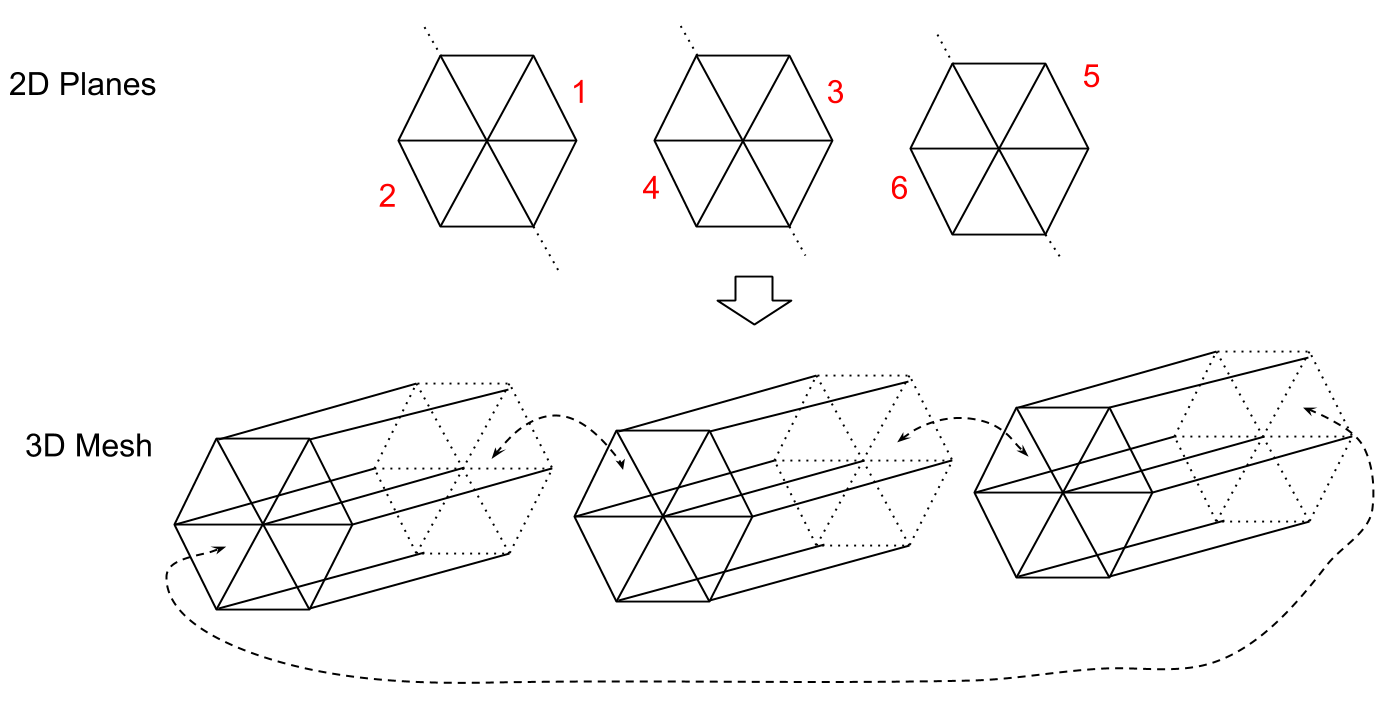
\includegraphics[width=0.8\textwidth]{fig/3dmesh.png}
\caption{The process of constructing 3D mesh. There are 6 processes and 3 planes. The dotted elements are remote copies at the mesh-part boundary (see \cite{pumi-web-page}).} \label{fig:3dmesh}
\end{figure}

\begin{figure}[htb]
\center
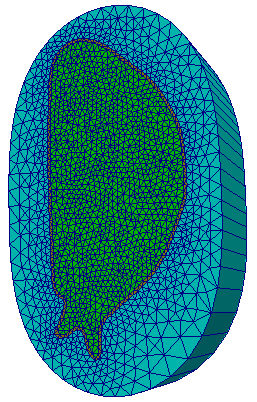
\includegraphics[width=0.5\textwidth]{fig/3dmeshSlice.png}
\caption{Wedge elements between planes} \label{fig:3dmeshSlice}
\end{figure}
\afterpage{\clearpage}
\section{Procedures to Interact with  Mesh Infrastructure} \label{sec:parallel}
This section discusses the procedures that interact between the underlying mesh infrastructure and the physics analysis code in M3D-C1 (Fig. \ref{fig:structure}).  The mesh infrastructure provides the information of the distributed mesh and the geometry that the mesh is classified on. Procedures that link  physics analysis code of M3D-C1 to the underlying mesh infrastructures  are developed. The procedures take the information from the mesh infrastructure and  compute the necessary inputs for use by the physics analysis. The procedure of mesh improvement through local modification also relies on the mesh infrastructure. The following paragraphs discuss the procedures that control the information flow between the mesh infrastructure and each specific component in M3D-C1.

The process of the PDE discretization over elements needs the information of the mesh entities and the geometric entities that the mesh entities are classified on. The procedure that inquires  the underlying mesh database and passes the information to the PDE discretization process is provided.  The mesh-entity-level information includes the connectivity of the element and the node position. The mesh-geometry classification identifies the set of the governing equation applied in a specific type of the region. The geometric shape such as the normal direction and curvature provides the necessary boundary information during the  PDE discretization process \cite{jardin2010computational}.

The process to form the global discrete equation needs the global DOF ordering and the procedure to assemble the global system of the equations. The global DOF ordering assigns a unique integer to the DOF's associated with mesh entities based on the mesh-adjacency information that improves the data locality \cite{zhou2010adjacency}. The parallel communication to assemble the global system of the equations is performed through the localized inter-process communication based on the mesh partition \cite{sahni2009strong,ovcharenko2012neighborhood}.  The connection and ownership between remote copies of mesh vertices \cite{Seol2014} at the part boundary is obtained form the mesh infrastructure and the elemental contribution to the stiffness matrix and the force vector is assembled by passing information between remote copies. Fig. \ref{fig:msgpassformat}.a illustrates the process. The non-owned vertices (hallowed circles) send the  the elemental contribution to the stiffness matrix and the force vector to owned vertices (solid circles) and the complete values are assembled.

\begin{figure}[htb]
\center
\begin{tabular}{cc}
%\subfloat[assemble]{\includegraphics[height=4cm]{fig/messagePassing2D.png}}
% & \subfloat[synchronize]{\includegraphics[height=4cm]{fig/messagePassing2DSyc.png}}
\end{tabular}
\caption{Inter-process communication between remote copies of mesh vertices. The mesh is partitioned into three parts and loaded by three processes. The dotted lines are boundaries of the mesh parts. The hollowed circles and dashed lines are non-owned mesh entities. The solid circles and lines are owned mesh entities. The arrows show the communication direction.} \label{fig:msgpassformat}
\end{figure}


There are procedures that set up the exterior  parallel equation solvers such as SuperLu \cite{superlu_ug99} and PETSc \cite{petsc-web-page} and return the solution vector to the analysis procedure. The owner vertices send the DOF's of the solution field to the non-owned vertices at the part boundary such that the solution field is synchronized. Fig. \ref{fig:msgpassformat}.b illustrates the process.

The assessment of the solution quality and mesh improvement needs interaction between the solution fields, mesh improvement procedure and the mesh infrastructure.  The correction indicator is calculated from the solution field and it is used to obtain the mesh size field that defines the optimal mesh desired.  The mesh is improved through local modifications \cite{li20053d,sahni2007automated, lu2013parallel} that interacts directly with the mesh infrastructure. Since the mesh is symmetric in the toroidal direction of the tokamak,  it is improved by adapting the 2D mesh on the cross section of the tokamak. The basic types of modifications on the 2D mesh include split, collapse, swap, node repositioning and snap. The mesh element can be refined by the split operation. The collapse operation can be used to coarsen the mesh. Element shapes can be improved by the operation of edge swap and node repositioning. Nodes classified on the geometric boundary are moved to the snapped position during mesh adaptation such that the consistency to the original geometry is maintained. These basic types of mesh modifications are further combined as the compound operations which provide more flexible ways to mesh improvement.

Solution fields on the original mesh can be easily transferred to the new mesh with the controlled error during the local mesh modification.  The process of solution transfer is to determine the DOF's of the field on the new mesh. The DOF's are attached to mesh vertices in M3D-C1 \cite{jardin2004triangular,jardin2012multiple} and correspond to the field value and its derivatives. New DOF's only need to be calculated when a new vertex is created during the operation of edge split or when a mesh vertex is moved during the operations of node repositioning and snap.  The field value and its derivatives on the original mesh are interpolated at the position of the new vertex or the position that the original vertex is moved to. The values of the new DOF's are obtained from the interpolated field value and its derivatives.

\section{Future Development in Mode Switch} \label{sec:futuredevelop}
\subsection{Mode Switch in M3D-C1} \label{sec:modeswitch}
 M3D-C1 studies the non-linear instability of plasma in the tokamak.  If the nonlinear instability is axis-symmetric, the equations are solved on a 2D mesh. In the situation of non-axis-symmetric instability, it needs to solve the equations on a 3D mesh. Currently, M3D-C1 runs in the following three modes.
\begin{itemize}
\item 2D with real numbers (\textit{2D Real})
\item 2D with complex numbers (\textit{2D Complex})
\item 3D with real numbers (\textit{3D Real})
\end{itemize}

In order to support the switch from \textit{2D Real} to \textit{3D Real},
M3D-C1 performs the \textit{2D Real}  simulation, and switch to the \textit{2D Complex} simulation periodically to check whether the non-axis-symmetric instability can happen. And then M3D-C1 switches from \textit{2D Real} to \textit{3D Real}.  The mesh changes from 2D to 3D and the solution of the field migrates from 2D mesh to 3D mesh. 

\subsection{Field In M3D-C1} \label{sec:field}
This section introduces the shape functions associated with the mesh element and the field interpolated by the shape functions in M3D-C1.

The 3D shape functions are defined by taking tensor product of the $C^1$ reduced quintic shape functions and the Hermite cubic polynomials \cite{jardin2004triangular,jardin2012review}.  The DOF's are listed in Table \ref{tab:dofs}.  The coordinate system is $(R,Z,\varphi)$ (Fig. \ref{fig:geo}).  DOF's of the $C^1$ triangle element  correspond to the function value, the first and second derivatives in the $R$ and $Z$ directions.  DOF's of the Hermite cubic polynomials correspond to the function value and the first derivative in the $\varphi$ direction.
\begin{table}
\begin{center}
 \begin{tabular}{|l|l|l|l|l|l|l|}
\hline
group 1 &$d$ & $d_{,R}$ & $d_{,Z}$ & $d_{,RR}$ & $d_{,RZ}$ &$d_{,ZZ}$  \\ \hline
group 2 &$d_{,\varphi}$ & $d_{,R\varphi}$ & $d_{,Z\varphi}$ & $d_{,RR\varphi}$ & $d_{,RZ\varphi}$ &$d_{,ZZ\varphi}$  \\ \hline
\end{tabular}
\caption{DOF's associated with the mesh vertex in M3D-C1} \label{tab:dofs}
\end{center}
\end{table}
A scaler field on the mesh with $N$ vertices is defined as
\begin{equation}
\sum_{i=1}^{NDOF} d_i \mu_i,
\end{equation}
where $d_i$ is the  $i^{th}$ DOF and  $\mu_i$ is the associated shape function. The number of DOF's, $NDOF$, is equal to $6N$ in the 2D mode that only the first group of DOF's in Table \ref{tab:dofs} are used, or is equal to $12N$ in the 3D mode. $d_i$ can either be a complex or real number.

The physics vector fields such as the velocity and the magnetic field are decomposed into scalar fields. For example, the velocity is decomposed into three scalar fields $(U, \omega, \chi)$ \cite{jardin2012multiple} is represented in the cylindrical coordinate $(R,Z, \varphi)$ as
\begin{equation}
\mathbf{V}=R^2\nabla U \times \nabla \varphi + R^2\omega\nabla\varphi+\frac{1}{R^2}\nabla_\perp\chi. \label{3scalars}
\end{equation}
In reduced models, the velocity is decomposed into less scalar fields in the form
\begin{equation}
\mathbf{V}=R^2\nabla U \times \nabla \varphi + R^2\omega\nabla\varphi 
\end{equation}
for the two scalar representation and
\begin{equation}
\mathbf{V}=R^2\nabla U \times \nabla \varphi.
\end{equation}
for the one scalar representation.

Currently, M3D-C1 can export and import the field data through the Adaptable IO System (ADIOS) (\url{https://www.olcf.ornl.gov/center-projects/adios/}). It allows M3D-C1 to check out the field data at some point (for example, running time hits the limit, system maintenance), and check in the data and continue the simulation later. It is a useful capability especially on the massively distributed computing systems that the chance of system failure increases. The √ of exporting and importing the field needs to happen within the same mode (see Sec. \ref{sec:modeswitch} for different modes in M3D-C1). 
\subsection{Future Development}
The future development lies in the following  aspects. 
\begin{enumerate}
\item mode control in M3D-C1. The mode in the physics code (M3D-C1) is controlled by passing different flags during the complication. If the mode needs to be switched during running time, the M3D-C1 needs to be reconstructed.

The SCOREC libraries control the mode by parameters in the functions and the mode can be changed during running time. 
\item a complete mesh representation of 3D mesh. The classification to the partition model needs to be properly maintained. A set of API functions in PUMI that supports modifying partition model during running time is under consideration. \footnote{The old way to change the partition model relies on the specific implementation of the partition model inside PUMI. It was abandoned as PUMI evolves. } 
\item field migration between the different modes through files or memories. The second type of switch needs to address the issue to map simulation results from 2D mesh to the 3D mesh.

 A high-level description of new functions needed  are listed as follows.
  
\begin{itemize}
\item
\begin{verbatim}
obtain_field( <in> vertexIdentifier,
             <in> planeIdentifier,
             <in> data_source,
             <out> buffer )
\end{verbatim}
Given the mesh vertex identifier and the plane identifier, obtain the field associated with the vertex and fill the data into the buffer. The data may come from memory (previous simulation results) or from file. For the first type switch,  the plane identifier is not needed since both modes are 2D (only one plane). 
\item
\begin{verbatim}
process_field ( <in> vertexIdentifier,
               <in> planeIdentifier,
               <inout> buffer )
\end{verbatim}
 Given the mesh vertex identifier and the plane identifier, process the associated field. In particular, the process adds perturbation to the field.
 \item
\begin{verbatim}  
feed_field ( <in> vertexIdentifier,
            <in> planeIdentifier,
            <in> buffer,
            <out>data_destination)
\end{verbatim}
The procedure feeds back the field associated with mesh vertex to the data destination. The data destination can be  memory if it is a restart of simulation, or file if it is a check point.
\end{itemize}
\end{enumerate}
\subsection{Options to Fulfill the New Capability During Running Time}
This sub section discusses the possible options to fulfill the new capability that migrates the field from 2D mesh to 3D mesh during running time.

The mesh and mesh partition is kept consistent in the 2D and 3D mesh during the mode switch. That is, the mesh on each plane in 3D mesh is the same as that in the 2D mesh.  The purpose is to avoid a global search of field data. Two options are described below.
\begin{itemize}
\item[1] The first option allows some processes to idle at some point (Fig. \ref{fig:wedgePlane}).  Allocate the processes that are need for the simulation on the 3D mesh. Assume there are $M$ planes, and each plane needs $N$ processes. The total number of processes allocated is $MN$. The processes are divided into $M$ groups.

The first group loads the 2D mesh and performs the 2D simulation. The rest groups of processes are just idling till the 3D simulation begins.

All the groups of processes obtain the mesh and field data from the first group that has been doing the 2D simulation. The 3D mesh is constructed by creating wedge elements between planes.  The 2D field data is processed by a pre-defined routine and then assigned to the 3D mesh. 
\begin{figure}[htb]
\center
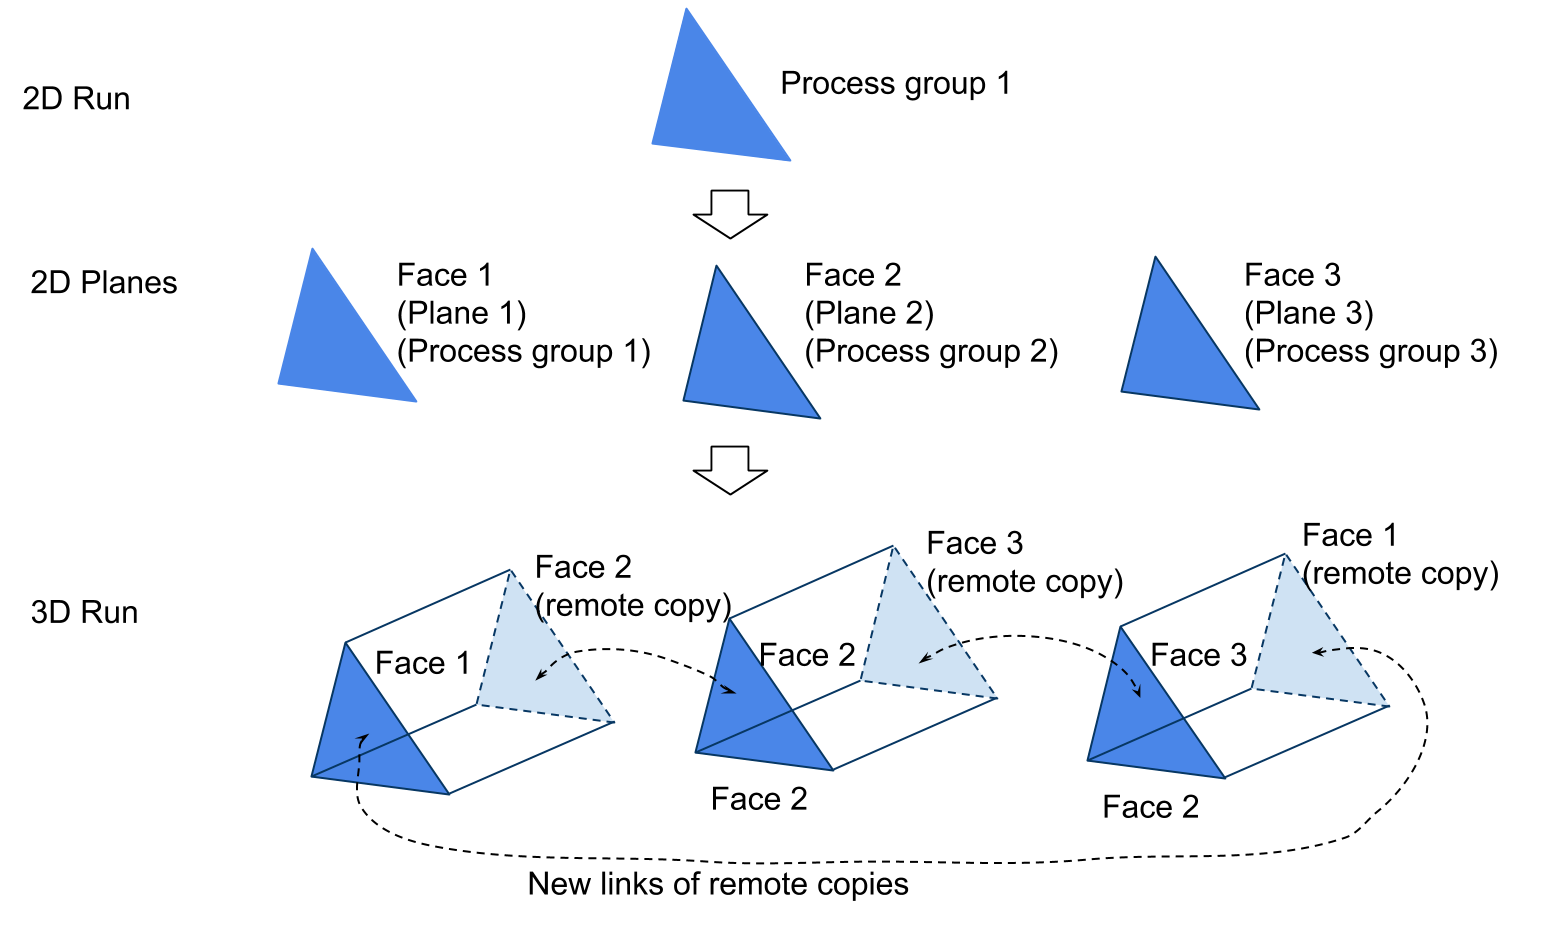
\includegraphics[width=0.8\textwidth]{fig/wedgePlane.png}
\caption{Option 1: idling processes. There are processes idling at the stage of 2D simulation.} \label{fig:wedgePlane}
\end{figure}
\item[2] The second option is to perform 2D simulation with all the processes (Fig. \ref{fig:wedgePlane2}).  Each process loads one part for 2D simulation.

In order to start 3D simulation,  the mesh part is migrated and each process holds multiple parts. For example, initially there are 6 processes that run on the 2D mesh and there are 6 parts of mesh. In order to start a 3D simulation with 3 planes, the mesh part is migrated and redistributed such that each process holds 3 parts of the mesh. Process 1 holds part 1, 2 and 3. Process 2 holds part 3, 4 and 5. Process 3 holds part 1,2,3. Process 3 holds part 4,5 and 6. And so on.

The field migrates with the mesh part.  The  3D mesh is constructed and the 2D field data is processed and assigned to the 3D mesh. 

\begin{figure}[htb]
\center
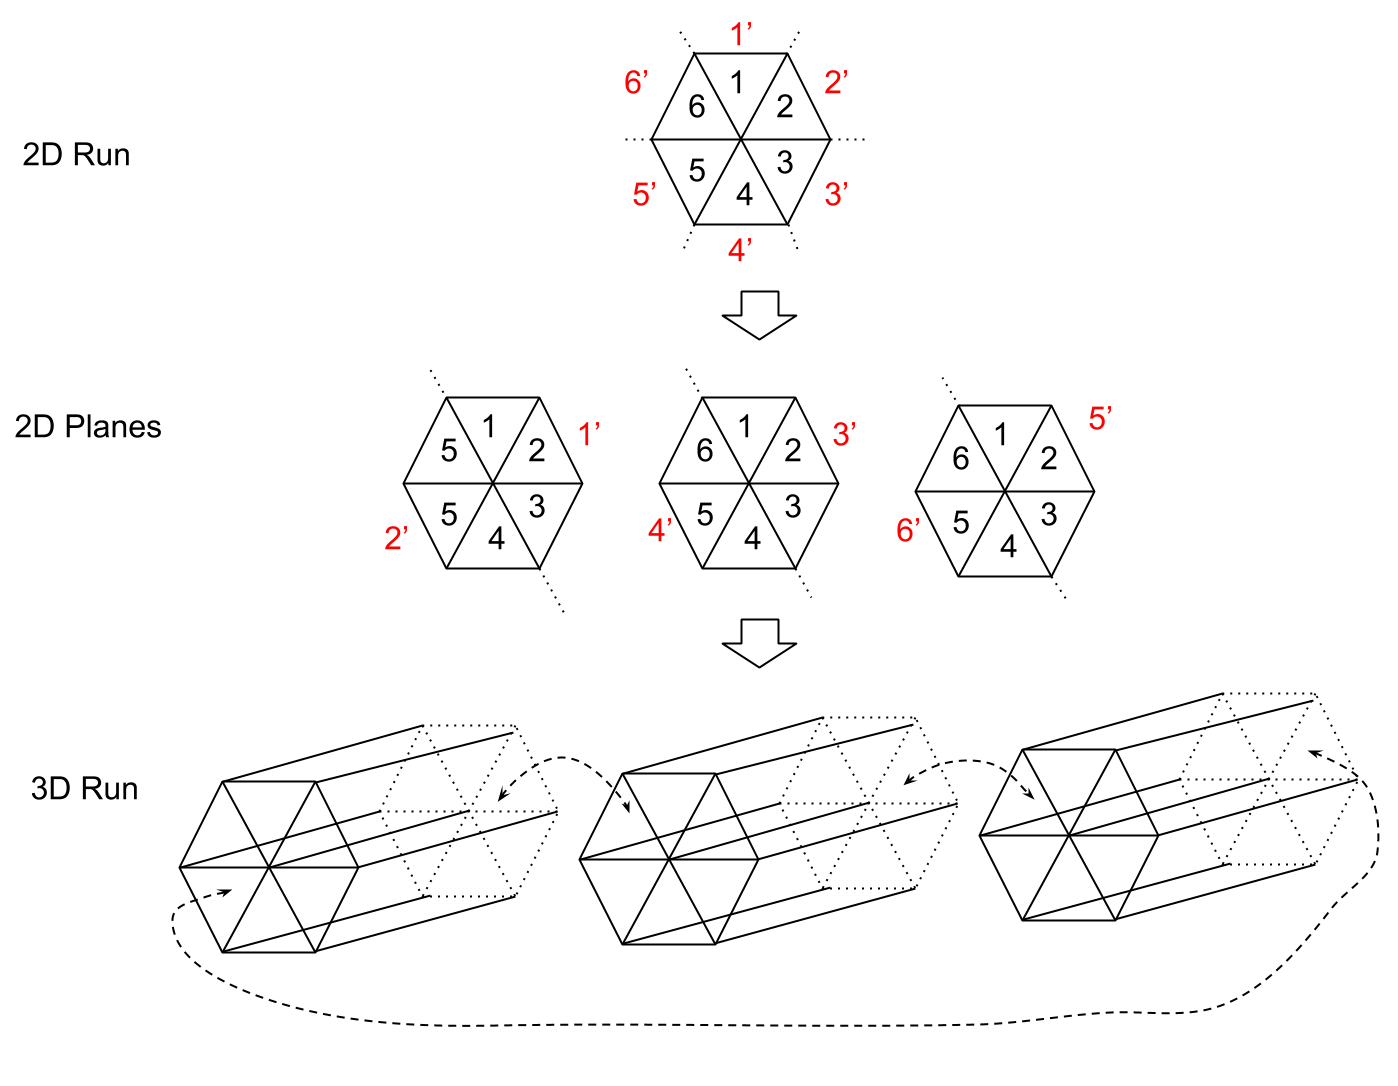
\includegraphics[width=0.8\textwidth]{fig/wedgePlane2.png}
\caption{Option 2: multiple parts on a single process. Each process holds 3 parts on the 3D mesh.} \label{fig:wedgePlane2}
\end{figure}
\end{itemize}

\clearpage
\bibliographystyle{ieeetr}
\bibliography{reference}
\clearpage
\appendix
\section{Software Components}
The following software components from SCOREC are used in M3D-C1.
\begin{itemize}
\item  Parallel Unstructured Mesh Management Infrastructure (PUMI) \cite{pumi-web-page}
\item \emph{MeshAdapt} that  provides services to support mesh topology modification
\end{itemize}

%Efforts to clean up codes are being performed.
%\begin{itemize}
%\item Removing unnecessary files/functions
%\item Replacing obsolete functions with PUMI functions. For instancen $PList$ and $FMDB$. 
%\item Eliminating global and unnecessarily duplicated variables
%\end{itemize}  
%%%%%%%%%%%%%%%%%%%%%%%%%%%%%%%
\section{Function list}
%%%%%%%%%%%%%%%%%%%%%%%%%%%%%%%
The section lists the functions provided to the M3D-C1 Fortran driver by SCOREC.The functions are declared in the file m3dc1$\_$scorec.h.
Throughout this section, unless specified,  mesh entities and DOF's are specified by a local ID. A word \emph{glob} is added to a function name to indicate a function that involves global communication or global data.

\subsection{Enumeration types}
The basic enumeration types that are used by the functions are listed. The coordinate system, the ordering option and the arithmetic type of  numbers are enumerated.

\begin{verbatim}
enum m3dc1_coord_system { /*0*/ M3DC1_RZPHI,  // default
                         /*1*/ M3DC1_XYZ};

enum m3dc1_ordering { 
  /*0*/ M3DC1_NO_ADJ=0,  // mesh element and DOF ordering use the order from mesh traversal - default
                         // solver (suplu_dist) reordering is turned on
  /*1*/ M3DC1_SERIAL_ADJ, // use adjaceny-based order from the serial mesh; 
                          // solver reordering is turned off        
  /*2*/ M3DC1_DISTR_ADJ, // use adjaceny-based order from the distributed mesh;
                         // solver reordering is turned off 
  /*3*/ M3DC1_DISTR_ADJ_SOLVER}; // use the adjaceny-based order from distributed
                                 // solver reordering is turned on

enum m3dc1_field_type { 
  /*0*/ M3DC1_REAL=0,  // real number for field value
  /*1*/ M3DC1_COMPLEX}; // complex number for field value
\end{verbatim}\vspace{-.5cm}\hspace{1cm}

\subsection{Initialization and finalization}
The functions that initializes and finalizes the usage of  the software are listed.
\begin{verbatim}
int m3dc1_domain_init();
\end{verbatim}\vspace{-.5cm}\hspace{1cm}

The function initializes the PUMI service for distributed model and mesh infrastructure. Note MPI should be initialized prior to this function.

\begin{verbatim}
int m3dc1_domain_finalize();
\end{verbatim}\vspace{-.5cm}\hspace{1cm}

The function finalizes the PUMI service and clears all model/mesh related data. Note MPI finalization is not included.

\begin{verbatim}
// old name: initsolvers_
int m3dc1_solver_init(); 
\end{verbatim}\vspace{-.5cm}\hspace{1cm}

The function initialize solver data structure.

\begin{verbatim}
// old name: finalizesolvers_
int m3dc1_solver_finalize()
\end{verbatim}\vspace{-.5cm}\hspace{1cm}

The function cleans the solver data structure. 

\subsection{Geometric model: general cross-section}
The functions that load the geometry description of the Tokamak cross section from the file and inquire the geometric model are listed.

\begin{verbatim}
int m3dc1_model_load (char*  /* in */  model_file);
\end{verbatim}\vspace{-.5cm}\hspace{1cm}

The function loads a geometric model from a model file that describe the geometry of the 2D cross section of the Tokamak. The file can contain
\begin{itemize}
\item parameters of the user specified analytic expression that defines a single loop as $R(t)=a_1 + a_2cos\left(t + a_3sin(t)\right)$ and $Z(t)= a_4 + a_5sin(t)$.
\item lists of geometric vertex and edges on the wall and vacuum boundaries and parameters of B-splines that define the shape of each edge.
\end{itemize}

\begin{verbatim}
// old name: setnbprocplane_
int m3dc1_model_setnumplane (int*    /* in */  num_plane);
\end{verbatim}\vspace{-.5cm}\hspace{1cm}

The function sets the number of planes to be used in the model.


\begin{verbatim}
// old name: setphirange_
int m3dc1_model_setphirange (
        double*  /* in */  min_val, 
        double*  /* in */  max_val);
\end{verbatim}\vspace{-.5cm}\hspace{1cm}

Given double values \emph{min\_val} and \emph{max\_val}, the function sets the phi range.

\begin{verbatim}
// old name: getmincoord2_
int m3dc1_model_getmincoord(
        double* /* out */ x_min, 
        double* /* out */ y_min);
\end{verbatim}\vspace{-.5cm}\hspace{1cm}

The function returns the minimum coordinate of the 2D cross section.
	      \textit{x\_min} is the minimum horizontal coordinate value. 
	      \textit{z\_min} is the minimum vertical coordinate value.
\begin{verbatim}
// old name getmaxcoord2_
int m3dc1_model_getmaxcoord (
        double* /* out */ x_max, 
        double* /* out */ y_max);
\end{verbatim}\vspace{-.5cm}\hspace{1cm}
        
The function returns the maximum coordinate of the 2D  cross section. 
          \textit{x\_max} is the maximum horizontal coordinate value. 
          \textit{Y\_max} is the maximum vertical coordinate value.

\subsection{Geometric model: rectangular cross section}
The functions that are only used when the cross section of the geometric model is rectangular are listed.

\begin{verbatim}
// old name: getmodeltags_
int m3dc1_model_getedge (
        int*  /* out */  left_edge,
        int*  /* out */  right_edge, 
        int*  /* out */  bottom_edge, 
        int*  /* out */  top_edge);

\end{verbatim}\vspace{-.5cm}\hspace{1cm}

The function returns the four model edges of the rectangular domain.

\begin{verbatim}
// old name: setperiodicinfo_
int m3dc1_model_setpbc (
        int* /* in */ x_pbc, 
        int* /* in */ y_pbc); 
\end{verbatim}\vspace{-.5cm}\hspace{1cm}

The function sets the periodic boundary condition in $x$ or $y$ direction of the rectangular domain. If the periodic boundary condition is used, set $x\_pbc$ or $y\_pbc$ to 1 (default: 0).
\begin{verbatim}
// old name: getperiodicinfo_
int m3dc1_model_getpbc (
        int* /* out */ x_pbc, 
        int* /* out */ y_pbc); 
\end{verbatim}\vspace{-.5cm}\hspace{1cm}

The function returns 1 (yes) or 0 (no) for the periodic boundary condition applied in $x$ or $y$ direction of the rectangular domain.
\subsection{Mesh}
The functions that load the mesh and inquire the mesh are listed.

\begin{verbatim}
int m3dc1_mesh_load (
        char*  /* in */  mesh_file, 
        int*   /* in */  distributed);
\end{verbatim}\vspace{-.5cm}\hspace{1cm}
 
The function loads a mesh from a mesh file.  \textit{distributed} is to indicate whether the input mesh is partitioned. The number of processes are divided into $num\_plane$ groups and each group loads the same 2D mesh.  $num\_plane$ is set by the function int $m3dc1\_model\_setnumplane$.
 
\begin{verbatim}
int m3dc1_mesh_build3d ();
\end{verbatim}\vspace{-.5cm}\hspace{1cm}
 
The function construct 3D mesh from 2D meshes loaded on multiple planes. If the number of plane is 1, the error code \emph{PUMI\_NOT\_SUPPORTED} is returned.

\begin{verbatim}
int m3dc1_mesh_setcoord(int* coord_system);
\end{verbatim}\vspace{-.5cm}\hspace{1cm}

The function sets the coordinate system. Use enumeration type \emph{m3dc1\_coord\_system}.

\begin{verbatim}
int m3dc1_mesh_getcoord(int* coord_system);
\end{verbatim}\vspace{-.5cm}\hspace{1cm}

The function returns the current coordinate system. 


\begin{verbatim}
 // old name  numnod_ ;
int m3dc1_mesh_getnument (
        int* /* in*/ ent_dim, 
        int* /* out */ num_ent);
\end{verbatim}\vspace{-.5cm}\hspace{1cm}

Given an entity dimension (0-3), the function gets the number of all (owned and not-owned) entities \textit{num\_ent} of the mesh on local process.
If $ent\_dim$ is not valid, the error code $PUMI\_INVALID\_ENTITY\_TYPE$ is returned.

\begin{verbatim}
 // old name: numownedents_
int m3dc1_mesh_getnumownent (
        int* /* in*/ ent_dim, 
        int* /* out */ num_ent);
\end{verbatim}\vspace{-.5cm}\hspace{1cm}

Given an entity dimension (0-3), the function gets the number of owned entities \textit{num\_ent} of the mesh on local process.
If $ent\_dim$ is not valid, the error code $PUMI\_INVALID\_ENTITY\_TYPE$ is returned.

\begin{verbatim}
 // old name: numglobalents_
int m3dc1_mesh_getnumglobent (
        int* /* in*/ ent_dim, 
        int* /* out */ global_num_ent);
\end{verbatim}\vspace{-.5cm}\hspace{1cm}

Given an entity dimension (0-3), the function gets the number of owned entities \textit{global\_num\_ent} of all processes.
If $ent\_dim$ is not valid, the error code $PUMI\_INVALID\_ENTITY\_TYPE$ is returned.

\begin{verbatim}
// old name: set_adj_ordering_
int m3dc1_mesh_setorderingopt (int* /* in */ option);
\end{verbatim}\vspace{-.5cm}\hspace{1cm}

The function sets the option for ordering. Use enumeration type \emph{m3dc1\_ordering} for the ordering option.
\begin{itemize}
\item M3DC1\_NO\_ADJ (or 0): use the ordering from mesh traversal (default)
\item M3DC1\_SERIAL\_ADJ (or 1): use the adjaceny-based ordering on the serial mesh.
\item M3DC1\_DISTR\_ADJ (or 2): adjacent ordering on the distributed mesh.
\item M3DC1\_DISTR\_ADJ\_SOLVER (or 3): combination of adjaceny-based ordering on the distributed mesh and the ordering from the solver.
\end{itemize} 

\begin{verbatim}
// old name: get_adj_ordering_option_
int m3dc1_mesh_getorderingopt (int* /* out */ option)
\end{verbatim}\vspace{-.5cm}\hspace{1cm}

The function gets the ordering option. 

\begin{verbatim}
// old name: createdofnumbering_
int m3dc1_mesh_setdofid (
        int* /* in */ dof_numbering_id, 
        int* /* in */ iper, 
        int* /* in */ jper,
        int* /* in */ num_dofs_per_vertex, 
        int* /* reserved - in */ num_dofs_per_edge,
        int* /* reserved - in */ num_dofs_per_face, 
        int* /* reserved - in */ num_dofs_per_region); 
\end{verbatim}\vspace{-.5cm}\hspace{1cm}

The function generates local and global DOF id's specified by \textit{dof\_numbering\_id}. \textit{do\_numbering\_id} should be a positive integer. The number of DOF's per mesh entity type is specified by \textit{num\_dofs\_per\_vertex}, \textit{num\_dofs\_per\_edge}, \textit{num\_dofs\_per\_face}, and \textit{num\_dofs\_per\_region}. Currently, the dof is supported only for vertex type. \textit{iper} and \textit{jper} indicate whether to use periodic boundary condition (PBC).
\begin{verbatim}
// old name: deletedofnumbering_
int m3dc1_mesh_deldofid (int* /* in */ dof_numbering_id); 
\end{verbatim}\vspace{-.5cm}\hspace{1cm}

The function deletes the DOF ordering specified by \textit{dof\_numbering\_id}. 

\begin{verbatim}
// old name: procdofs_
int m3dc1_mesh_getdofid (
        int* /* in */ dof_numbering_id, 
        int* /* out */ start_dof_id, 
        int* /* out */ end_dof_id_plus_one); 
\end{verbatim}\vspace{-.5cm}\hspace{1cm}

The function gets the starting local DOF id and ending local DOF id + 1. 

\begin{verbatim}
// old name: procdofs_
int m3dc1_mesh_getglobdofid (
        int* /* in */ dof_numbering_id, 
        int* /* out */ start_glob_dof_id, 
        int* /* out */ end_glob_dof_id_plus_one); 
\end{verbatim}\vspace{-.5cm}\hspace{1cm}

The function gets the global start DOF id and end DOF id plus one. Each process owns a consecutive piece of DOF's ordered globally. 

\begin{verbatim}
// old name: numdofs_
int m3dc1_mesh_getnumdof (
        int* /* in */ dof_numbering_id, 
        int* /* out */ num_local_dofs); 
\end{verbatim}\vspace{-.5cm}\hspace{1cm}
 
The function gets the number of DOF's (owned and unowned) on local process in the DOF orderings specified by \textit{dof\_numbering\_id}. 

\begin{verbatim}
\\ old name: numglobaldofs_
int m3dc1_mesh_getnumglobdof (
        int* /* in */ dof_numbering_id, 
        int* /* out */ num_global_dof);
\end{verbatim}\vspace{-.5cm}\hspace{1cm}

The function returns the global number of the DOF's specified by \textit{dof\_numbering\_id}.  

\begin{verbatim}
// old name: numprocdofs_
int  m3dc1_mesh_getnumowndof (
        int* /* in */ dof_numbering_id, 
        int* /* out */ num_own_dof);
\end{verbatim}\vspace{-.5cm}\hspace{1cm}

The function gets the number of owned DOF's on local process. 

\subsection{Mesh Improvement by adaptation}
The functions that improve the mesh by adaptation are listed.
\begin{verbatim}
// old name: setsmoothfact_
int  m3dc1_mesh_setsmoothftr (double* /* in */ fact)
\end{verbatim}\vspace{-.5cm}\hspace{1cm}

The function sets the smooth factor of the size field that drives the mesh adaptation.

\begin{verbatim}
// old name: adapt_
int  m3dc1_mesh_adapt (
        double* /* in */ vecid, 
        double* /* in */ psi0,  
        double* /* in */ psil); 
\end{verbatim}\vspace{-.5cm}\hspace{1cm}

The function adapts the mesh by the analytic size field defined in terms of  the solution field. The parameters in the analytic expression are defined in the file sizefieldParam.
	      \textit{vecid} is is the solution field. 
	      \textit{psi0} and \textit{psil} are two parameters to normalize the field value. 
	      The normalized field value is $\bar{psi} = (psi - *psi0)/(*psil - *psi0)$.


\subsection{Mesh entity}
The functions that inquire the mesh entity (a vertex, a edge, a face or a region) are listed. The mesh entity is specified by a local ID and the dimension.
\begin{verbatim}
// old name: zonfac_
int m3dc1_ent_getgeomclass ( 
        int* /* in */ ent_dim, 
        int* /* in */ ent_id, 
        int* /* out */ geom_class_dim, 
        int* /* out */ geom_class_id); 
\end{verbatim}\vspace{-.5cm}\hspace{1cm}

Given entity's dimension and local id, the function gets the dimension and id of geometric entity that the mesh entity is classified on. If entity dimension and id are not valid, the error code $PUMI\_INVALID\_ENTITY\_HANDLE$ is returned.

\begin{verbatim}
// old name: functions that inquire adjacent entities
int m3dc1_ent_getadj (
        int* /* in */ ent_dim, 
        int* /* in */ ent_id, 
        int* /* in */ adj_dim,
        int*/* inout */ adj_ent,
        int* /* in */ adj_ent_allocated_size,
        int* /* out */ num_adj_ent); 
\end{verbatim}\vspace{-.5cm}\hspace{1cm}

Given entity's dimension and local id, and entity type for adjacency, the function gets the local ids' and the size of adjacenct entities. \emph{adj\_ent} is an array representing adjacent entitites' local id and \emph{adj\_ent\_allocated\_size} and \emph{adj\_ent\_size} represent the size of memory allocated to \emph{adj\_ent} and the size of adjacent entities, respectively. If \emph{adj\_ent\_allocated\_size} is less than \emph{adj\_ent\_size}, the error code \emph{PUMI\_BAD\_ARRAY\_SIZE} is returned. If entity dimension, id or $adj\_dim$ is not valid, the error code $PUMI\_INVALID\_ARGUMENT$ is returned. If entity's local id is not available, the error code \emph{PUMI\_FAILURE} is returned.
	      
\begin{verbatim}
// old name: functions that inquire number of adjacent entities
int m3dc1_ent_getnumadj (
        int* /* in */ ent_dim, 
        int* /* in */ ent_id, 
        int* /* in */ adj_dim,
        int* /* out */ num_adj_ent);
\end{verbatim}\vspace{-.5cm}\hspace{1cm}

Given entity's dimension and local id, and entity type for adjacency, the function gets the number of adjacenct entities. If entity dimension and id are not valid, the error code $PUMI\_INVALID\_ENTITY\_HANDLE$ is returned. If $adj\_dim$ is not valid, the error code \emph{PUMI\_INVALID\_ARGUMENT} is returned. 


\begin{verbatim}
// old name: entprocowner_
int m3dc1_ent_getpartid_own (
        int* /* in */ ent_dim, 
        int* /* in */ ent_id, 
        int* /* out */ owning_partid); 
\end{verbatim}\vspace{-.5cm}\hspace{1cm}

Given entity's dimension and local id, the function gets the owning part id. If entity dimension and id are not valid, the error code \emph{PUMI\_INVALID\_ENTITY\_HANDLE} is returned.

\begin{verbatim}
// old name: globalidnod_
int m3dc1_ent_getglobid (
        int* /* in */ ent_dim, 
        int* /* in */ ent_id, 
        int* /* out */ glob_ent_id); 
\end{verbatim}\vspace{-.5cm}\hspace{1cm}

Given entity's dimension and local id, the function gets the global id of the entity. If entity dimension and id are not valid, the error code \emph{PUMI\_INVALID\_ENTITY\_HANDLE} is returned. If entity's global id is not available, the error code \emph{PUMI\_FAILURE} is returned.


\begin{verbatim}
int m3dc1_ent_getnumdof (
       int* /* in */ ent_dim, 
       int* /* in */ ent_id, 
       int* /* out */ num_dof);
\end{verbatim}\vspace{-.5cm}\hspace{1cm}
Given entity's dimension and local id, the function gets the number of DOF's associated with the entity.

\begin{verbatim}
// old name: entdofs_
int m3dc1_ent_getdofid(
        int* /* in */ dof_numbering_id, 
        int* /* in */ ent_dim, 
        int* /* in */ ent_id, 
        int* /* out */ start_dof_id, 
        int* /* out */ end_dof_id_plus_one); 
\end{verbatim}\vspace{-.5cm}\hspace{1cm}
 
Given entity's dimension and local id, the function gets the local start DOF id \textit{start\_dof\_id} and the local end DOF id \textit{end\_dof\_id\_plus\_one} specified by \textit{dof\_numbering\_id}. 

\begin{verbatim}
// old name: globalentdofs_
int m3dc1_ent_getglobdofid(
        int* /* in */ dof_numbering_id, 
        int* /* in */ ent_dim, 
        int* /* in */ ent_id, 
        int* /* out */ start_glob_dof_id, 
        int* /* out */ end_glob_dof_id_plus_one); 
\end{verbatim}\vspace{-.5cm}\hspace{1cm}
 
Given entity's dimension and local id, the function gets the starting global DOF id \textit{start\_glob\_dof\_id} and the ending global DOF id + 1 \textit{end\_glob\_dof\_id\_plus\_one} specified by \textit{dof\_numbering\_id}. 

\subsection{Mesh Vertex}
The functions that inquire the mesh vertex are listed.
\begin{verbatim}
// old name: xyznod_
int m3dc1_vertex_getcoord (
        int* /* in */ node_id , 
        double* /* out */ coord ); 
\end{verbatim}\vspace{-.5cm}\hspace{1cm}
Given local node id, the function gets the coordinate of the mesh vertex in the arrary \textit{coord}. 
The size of \textit{coord} is 3. For a 2D mesh, the value of $coord[2]$ is 0.0. If no node exists for $node\_id$, the error code \emph{PUMI\_INVALID\_ENTITY\_HANDLE} is returned. If $adj\_dim$ is not valid, the error code \emph{PUMI\_INVALID\_ARGUMENT} is returned. 

\begin{verbatim}
// old name: nodnormalvec_
int m3dc1_vertex_getnormvec (
        int* /* in */ node_id, 
        double* /* out */ xyz);
\end{verbatim}\vspace{-.5cm}\hspace{1cm}

    The function gets the normal vector for a boundary mesh vertex \textit{node\_id} defined on a 2D plane

\begin{verbatim}
// old name: nodnormalvec_
int m3dc1_vertex_isongeombdry (int* /* in */ node_id, int* /* out */ on_geom_bdry)
\end{verbatim}\vspace{-.5cm}\hspace{1cm}

    The function gets an integer indicating whether the input node is on the geometric boundary (1) or not (0).

\subsection{Field}
The functions that creates and perform the parallel assembly and synchronization of  a field are listed. 
\begin{verbatim}
// old name: createppplvec_
int m3dc1_field_create (
        double* /* in */ field_id, 
        int* /* in */ dof_numbering_id, 
        int* /* in */ field_type); 
\end{verbatim}\vspace{-.5cm}\hspace{1cm}

The function creates a field (vector) with ID \textit{field\_id} from the DOF ordering \textit{dof\_numbering\_id}. Use enumberation type \emph{m3dc1\_field\_type} for \textit{field\_type}. Note the  memory for the field is allocated and freed by the Fortran driver.

\begin{verbatim}
// old name: deleteppplvec_
int m3dc1_field_delete (double* /* out */ field_id); 
\end{verbatim}\vspace{-.5cm}\hspace{1cm}

The function deletes the field specified by \textit{field\_id}.

\begin{verbatim}
// old name: checkppplveccreated_
int m3dc1_field_exist(
        double* /* in */ field_id, 
        int* /* out */ iscreated);/
\end{verbatim}\vspace{-.5cm}\hspace{1cm}

The function checks if the field specified by \textit{field\_id} is created.

\begin{verbatim}
int m3dc1_field_sync (double* /* in */ field_id); 
\end{verbatim}\vspace{-.5cm}\hspace{1cm}

When the values of the DOF's are obtained by  integration over elements, the values are incomplete at the part boundary. The function performs parallel assembly and synchronize of the field on the part boundary by sending the field of non-owned mesh entities to the owner mesh entities. The values are summed up at the owner entities and sent back to the non-owned entities.  

\begin{verbatim}
// old name: updatesharedppplvecvals_;
int m3dc1_field_sync (double* /* in */ id); 
\end{verbatim}\vspace{-.5cm}\hspace{1cm}

The function performs synchronize of the field on the part boundary. The field values of the owner nodes are sent to the non-owned nodes and the values of the field on the part boundary is synchronized to have the value.  

\begin{verbatim}
// old name: updateids_
int m3dc1_field_changeid (
        double* /* in */ old_field_id, 
        double* /* in */ new_field_id); 
\end{verbatim}\vspace{-.5cm}\hspace{1cm}

The function updates the field ID.

\begin{verbatim}
// old name: sum_vec_planes_
int m3dc1_field_getsumofplane (double* /* in */ thevec); 
\end{verbatim}\vspace{-.5cm}\hspace{1cm}

The function sums up the values of the field over the planes. The field of the mesh nodes with same $(R,Z)$ coordinate on different planes are summed. 

\subsection{Solution Transfer}
The functions that transfer the solution fields from the original mesh to the new mesh during mesh adaptation are listed. 
\begin{verbatim}
// old name: initSolutionTransfer_
int m3dc1_fieldtransfer_init(int* /* in */ option); 
\end{verbatim}\vspace{-.5cm}\hspace{1cm}

The function initiates the solution transfer before mesh is adapted.

\begin{verbatim}
// old name: registerFieldTransfer_
int m3dc1_fieldtransfer_register ( 
        double* /* in */ inputField, 
        const char* /* in */ key); 
\end{verbatim}\vspace{-.5cm}\hspace{1cm}

The function register the field that needs to be transferred during mesh adaptation.

\begin{verbatim}
// old name: finalizeSolutionTransfer_
int m3dc1_fieldtransfer_finalize ();
\end{verbatim}\vspace{-.5cm}\hspace{1cm}

The function finalizes the field  transfer after mesh adaptation.

\begin{verbatim}
// old name: getFieldTransfer_
int m3dc1_fieldtransfer_get (
        double* /* out */ inputField, 
        const char* /* in */ key); 
\end{verbatim}\vspace{-.5cm}\hspace{1cm}
The function returns the transfered field on the adapted mesh. 
\begin{verbatim}
// old name: deleteSolutionTransfer_
int m3dc1_fieldtransfer_delete(); 
\end{verbatim}\vspace{-.5cm}\hspace{1cm}

The function deletes the field transfer object.
\subsection{Matrix}
The functions that form and solve the global discrete equation are listed.
\begin{verbatim}
// old name: zerosuperlumatrix_ zeropetscmatrix_ zeromultiplymatrix_
int m3dc1_matrix_init (
        int* /* in */ matrixid,
        int* /* in */ matrixType,
        int* /* in */ valtype,  
        int* /* in */ dof_numbering_id); 
\end{verbatim}\vspace{-.5cm}\hspace{1cm}

The function initiates  the matrix with ID \textit{matrixid} that uses the DOF ordering \textit{dof\_numbering\_id} 
	       for use with the matrix.
	       matrixType indicates the purpose of the matrix. matrixType=0 for matrix-vector multiplication, matrixType=1 for superlu solver, matrixType=2 for petsc solver.
	       If the real numbers are 	used,  set \textit{type} to 0.
	       If the complex numbers are used,  set \textit{type} to 1. 
	       If the matrix has already been created then it just cleans out the matrix.

	       
\begin{verbatim}
// old name: insertval_
int m3dc1_matrix_insertval (
        int* /* in */ matrixid, 
        double* /* in */ val, 
        int* /* in */ valtype, 
        int* /* in */ row,
        int* /* in */ column, 
        int* /* in */ operation); 
\end{verbatim}\vspace{-.5cm}\hspace{1cm}

The function inserts \textit{val} to matrix \textit{matrixid}
	       at (\textit{row},\textit{column}).
	       \textit{row} and \textit{column} come from the DOF ordering associated with the matrix.
	       The type of value to be inserted can be real (\textit{valtype} =0) or complex (\textit{valtype}=1).
	       A real type can be inserted into a complex matrix
	       but a complex type cannot be inserted into a real matrix.
	       If \textit{operation} is zero then the value overwrites any existing value,
	       otherwise the value is to be added to the existing value.

\begin{verbatim}
// old name: globalinsertval_
int m3dc1_matrix_globalinsertval (
        int* /* in */ matrixid, 
        double* /* in */ val, 
        int* /* in */ valtype, 
        int* /* in */ row,
        int* /* in */ column, 
        int* /* in */ operation); 
\end{verbatim}\vspace{-.5cm}\hspace{1cm}

The function inserts \textit{val} into matrix \textit{matrixid} at
	       (\textit{globalrow}, \textit{globalcolumn}) in the matrix 
	       where \textit{globalrow} and \textit{globalcolumn} are defined as the global labels of the DOF.
	       \textit{globalrow} needs to correspond to a local DOF.
	        \textit{globalcolumn} can either  correspond to a local DOF or a node locate on the geometric boundary.

\begin{verbatim}
int m3dc1_matrix_setdiribc(
        int* /* in */ matrixid, 
        int* /* in */ row);
\end{verbatim}\vspace{-.5cm}\hspace{1cm}
	       
The function zeroes out all off-diagonal values in the \textit{row}  of  matrix \textit{matrixid}
	       and sets the diagonal value to be one.
	       The operation is carried out during finalizing the matrix, 
	       This function will overwrite other insertion operations to the row.
	       For complex-valued arrays,
	       the real part of the diagonal is set to be one and the imaginary part is set to zero.
	       This function should be called on all processes that use the DOF number associated with the matrix row.

\begin{verbatim}
int m3dc1_matrix_setgeneralbc_ (
        int* /* in */ matrixid, 
        int* /* in */ row, 
        int* /* in */ numvals,
        int* /* in */ columninfo, 
        double* /* in */ vals, 
        int* valtype);
\end{verbatim}\vspace{-.5cm}\hspace{1cm}

 The function sets multiple values for the row of \textit{matrixid}.
	       The  number of values to be inserted is \textit{numvals}. 
	       \textit{columninfo} specifies which columns to set the values and 
	       and \textit{vals} specifies the values to be set
	       which must be in the same order as the \textit{columninfo} array.
	       The type of values to be inserted can be real (\textit{type} =0) or complex (\textit{type} =1).
	       If only real values are inserted into a complex matrix,
	       then the corresponding imaginary parts are set to zero. 
	       The operation is carried out during finalizing the matrix, 
	       This function will overwrite other insertion operations to the row.
	       This function should be called on all processes that use the DOF number associated with the matrix row.

\begin{verbatim}
// old name: finalizematrix_
int m3dc1_matrix_finalize (int* /* in */ matrixid); 
\end{verbatim}\vspace{-.5cm}\hspace{1cm}

The function finalizes \textit{matrixid} such that no more values can be inserted into the matrix 
	       and no more boundary conditions can be applied to the matrix.

\begin{verbatim}
// old name: solveSysEqu_
int m3dc1_matrix_solve (
        int* /* in */ matrixid, 
        double* /* inout */ rhs_sol, 
        int* /* out */ ier); 
\end{verbatim}\vspace{-.5cm}\hspace{1cm}
 
 The function solves the linear systems of equation $Ax=b$. The matrix $A$ is created by \textit{m3dc1\_matrix\_initsuperlu} or \textit{m3dc1\_matrix\_initpetsc} , 
The input right-hand-side vector \textit{rhs\_sol} is overwritten with the solution.
	       If \textit{ier} is non-zero there were mistakes returned by the solver. 
\begin{verbatim}
// old name: matrixvectormult_
int m3dc1_matrix_multiplyvec (
        int* /* in */ matrixid, 
        double* /* in */ inputvecid, 
        double* /* out */ outputvecid); 
\end{verbatim}\vspace{-.5cm}\hspace{1cm}

The function performs the matrix-vector multiplication. Matrix
\textit{matrixid} is created by \textit{m3dc1\_matrix\_initmultiply}.
	       If either \textit{matrixid} or \textit{inputvecid} is complex-valued,
	       \textit{outputvecid} must also be complex-valued.

\begin{verbatim}
// old name: deletematrix_
int m3dc1_matrix_delete (int* /* in */ matrixid); 
\end{verbatim}\vspace{-.5cm}\hspace{1cm}

The function deletes the matrix.

\begin{verbatim}
// old name: writematrixtofile_
int m3dc1_matrix_write (
        int* /* in */ matrixid, 
        int* /* in */ fileid, 
        int* /* in */ option); 
\end{verbatim}\vspace{-.5cm}\hspace{1cm}

The function writes the matrix to the file. If \textit{option==1}, the imaginary and real parts of the matrix are outputted to separated files.




\section{Verification Tools} \label{sec:test}
Table~\ref{tab:fusion-test} illustrates available tests using only SCOREC software. The sample meshes and models can be found under the folder $yourCodeRoot/meshes/$. Table~\ref{tab:fusion-test-m3dc1} illustrates M3D-C1 tests for verification purpose. Notice that smaller meshes are used in M3D-C1 tests for  verification purpose.


\begin{table}
\begin{center}
\caption{Available M3D-C1 Tests (SCOREC software only)}
\label{tab:fusion-test}
%\begin{tiny}
\begin{tabular}{l|p{11cm}}
\hline
  {\bf Test Program}  &  {\bf Description}  \\

\hline
   test/DEMO3DCurved & 

\multicolumn{1}{|c} {
 \begin{minipage}[t]{4.5in} \raggedright
  $\bullet$ Purpose: build the 3D mesh from 2D mesh\\
  $\bullet$ Arguments: mpirun -np np ./main numPlane  numProcPerPlane model\\
  $\bullet$ Input mesh: the 2D mesh partitioned into numProcPerPlane parts by test/PTNMESH\\
  
  $\bullet$ Results: output normal directions and curvatures at the geometry boundary; output vtu file to view the 3D mesh\\
 \end{minipage}
 } \\

\hline
   test/SumInfo & 

\multicolumn{1}{|c} {
 \begin{minipage}[t]{4.5in} \raggedright
  $\bullet$ Purpose: test parallel communication between remote copies of mesh vertices and dofs\\
  $\bullet$ Arguments: mpirun -np np ./main model mesh numPlane numProcPerPlane \\
  $\bullet$ Input mesh/model: for 2D mesh, set numPlane=1;  for 3D mesh,  the input is a 2D mesh partitioned into numProcPerPlane parts and set numPlane larger than 1.\\
  
  $\bullet$ Results: if success, the program terminates normally; else, error message is output.\\
 \end{minipage}
 } \\
\hline

   test/RWBTest & 

\multicolumn{1}{|c} {
 \begin{minipage}[t]{4.5in} \raggedright
  $\bullet$ Purpose: test 2D resistive wall boundary condition; test elemental routines of matrix and vector; test solver interfaces. \\
  $\bullet$ Arguments: mpirun -np np ./main model mesh solverOption \\
  $\bullet$ Input mesh/model: cp meshes/mesh1/* .\\
       solverOption: 0 uses SuperLu; 1 uses PETSc. \\
  $\bullet$ Results: if success, the program terminates normally; else, error message is output.\\
 \end{minipage}
 } \\
\hline

   test/adapt\_fn & 

\multicolumn{1}{|c} {
 \begin{minipage}[t]{4.5in} \raggedright
  $\bullet$ Purpose: test 2D adaptation on the analytical model. \\
  $\bullet$ Arguments: ./main model mesh \\
  $\bullet$ Input mesh/model: cp meshes/mesh2/* .\\
  $\bullet$ Results: output an adapted mesh adapted.sms \\
 \end{minipage}
 } \\
\hline
   test/PTNMESH& 

\multicolumn{1}{|c} {
 \begin{minipage}[t]{4.5in} \raggedright
  $\bullet$ Purpose:  perform 2D mesh partition \\
  $\bullet$ Arguments: mpirun -np np ./main mesh \\
  $\bullet$ Input mesh: /path/to/model/mesh/files\\
  $\bullet$ Results: the 2D mesh is partitioned into np parts.\\
 \end{minipage}
 } \\

\hline
\end{tabular}
%\end{tiny}
\end{center}
\end{table}
 

\begin{table}
\begin{center}
\caption{Available M3D-C1 Tests}
\label{tab:fusion-test-m3dc1}
%\begin{tiny}
\begin{tabular}{l|p{11cm}}
\hline
  {\bf Test Program}  &  {\bf Description}  \\

\hline
   DATA/CMODTearing & 

\multicolumn{1}{|c} {
 \begin{minipage}[t]{4.5in} \raggedright
  $\bullet$ Purpose: test 2D real M3DC1\\
  $\bullet$ Build flags:  make\\
  $\bullet$ Arguments: mpirun -np 8 ../../\_twister-25/m3dc1\\
  $\bullet$ Results:  To verify code cleanup, compare if the same C1ke file is obtained. \\
 \end{minipage}
 } \\

\hline
   DATA/3DNL-4planes8p & 

\multicolumn{1}{|c} {
 \begin{minipage}[t]{4.5in} \raggedright
  $\bullet$ Purpose: test 3D real M3DC1\\
 $\bullet$ Build flags:  make 3D=1 \\
  $\bullet$ Arguments: mpirun -np 8 ../../\_twister-25/m3dc1\\
  $\bullet$ Results:  To verify code cleanup, compare if the same C1ke file is obtained. \\
 \end{minipage}
 } \\
\hline

\end{tabular}
%\end{tiny}
\end{center}
\end{table}
\end{document}
